\documentclass[a4paper,12pt]{article}
\usepackage[utf8]{inputenc}
\usepackage[russian]{babel}
\usepackage{amssymb,amsmath,amsfonts,amsthm,amscd,latexsym,graphicx,epsfig,colordvi}
\usepackage[mag=1000,a4paper,left=1cm,right=1cm,top=0.5cm,bottom=0.5cm,noheadfoot]{geometry}
\usepackage{graphics}
\usepackage{arcs}
\usepackage{verbatim}
\usepackage{cmap}
\usepackage[T2A]{fontenc}

\setlength{\parskip}{0.5cm}

\pagestyle{empty}

\begin{document}

{\bf\Large  Быстрое преобразование Хафа}

{\bf Классическое преобразование Хафа}

{\it Преобразование Хафа}~--- алгоритм, применяемый для поиска на изображении параметрических кривых, чаще всего, прямых и окружностей. Данное преобразование является отображением из пространства изображения в пространство параметров кривой. Опишем классический алгоритм Хафа поиска прямых.

Зададим прямую на изображении двумя параметрами: $\rho$~--- расстояние от прямой до начала координат, $\varphi$~--- угол между внешней нормалью прямой и осью абсцисс. Уравнение прямой записывается через параметры $\rho, \varphi$ следующим образом: $$ x \cos\varphi + y \sin\varphi = \rho, $$ где $x, y$~--- координаты точки на изображении. Данное уравнение устанавливает отображение из множества прямых на изображении во множество точек плоскости параметров $(\rho,\varphi)$. С другой стороны, каждой точке $(x_0,y_0)$ на изображении соответствует синусоида в пространстве параметров, задаваемая этим же уравнением, причем каждая точка на этой синусоиде соответствует некоторой прямой, проходящей через $(x_0,y_0)$. Разделим пространство параметров на ячейки и свяжем с каждой ячейкой счетчик. Для каждой точки $(x_0,y_0)$ изображения построим синусоиду в пространстве параметров с яркостью, пропорциональной яркости точки изображения $(x_0,y_0)$, а затем увеличим счетчики ячеек, через которые прошла синусоида, на яркость синусоиды. Если счетчик ячейки с центром $(\rho_0,\varphi_0)$ является локальным максимумом, то на изображении есть много ярких точек, лежащих на прямой с параметрами, близкими к $(\rho_0,\varphi_0)$.

Однако изъян данного алгоритма заключается в высокой вычислительной сложности, которая составляет $O(n^3)$. Значительного улучшения можно добиться, используя алгоритм {\it быстрого преобразования Хафа (БПХ, FHT)}.

{\bf Быстрое преобразование Хафа. (s,t)-параметризация}

Введем $(s, t)$-параметризацию прямой на изображении, которая по существу аналогична классической параметризации. Введем два типа геометрических прямых: преимущественно-горизонтальные прямые (ПГП) и преимущественно-вертикальные прямые (ПВП). Угловой коэффициент первых лежит в диапазоне $|k| \leq 1$, а вторых~--- $|k| \geq 1$.

ПГП будем задавать параметрами $s$ и $t$ координат двух принадлежащих ей точек на вертикальных границах изображения: $(0, s)$ и $(n - 1, s + t)$, а ПВП~--- на горизонтальных: $(s, 0)$ и $(s + t, n - 1)$, где $t \in [-n + 1; n - 1]$ и $s \in [-n + 1; n - 1]$. Знак $t$ определяет направлением относительно координатной оси. Если $t \leq 0$, то такие прямые называются ПГП c наклоном вниз, если $t \geq 0$~--- с наклоном вверх. Без ограничения общности опишем далее только алгоритм поиска ПГП с наклоном вверх, поиск остальных трёх типов прямых осуществляется в точности аналогично.

{\bf Диадические паттерны}

При создании алгоритма БПХ был предложен так называемый диадический паттерн (ДП). Существует два способа задавать ДП~--- рекурсивный и аналитический. Для описанного далее алгоритма достаточно рекурсивного определения: \[P^n_t = P^{n/2}_{\lfloor t/2 \rfloor} \cup \Biggl( P^{n/2}_{\lfloor t/2 \rfloor)} \nearrow (n/2, \lfloor t/2 \rfloor + t\;mod\;2) \Biggr), \] где $P^j_i$~--- множество пикселей, принадлежащих паттерну с наклоном $i$ и длиной $j$, а стрелка обозначает приращение координат всех элементов множества на указанный вектор, причем $P^1_0 = \{(0, 0)\}$.

Опишем подробнее, что именно за правило описывает эта формула. На каждом шаге рекурсии изображение делится вертикально на две равные части, и для каждой из этих частей определяется наклон диадического подпаттерна и сдвиг (0 или 1) между ними. Эти значения задают координаты пикселей на границе разделения: $(n/2 - 1, \lfloor t/2 \rfloor)$ и $(n/2, \lfloor t/2 \rfloor + t\;mod\;2)$. Затем процедура проводится для каждого подпаттерна до тех пор, пока длина изображения не будет равна единице. Из определения видно, что диадический паттерн обладает самоподобной структурой. Используя данное определение, можно показать связь между битовым представлением наклона $t$ и структурой паттерна. Если в битовом представлении в $k$-м разряде стоит единица, значит на $k$-м шаге рекурсии каждая пара подпаттернов будет сдвинута на единицу относительно друг друга.

\begin{figure}[h!]
  \centering
  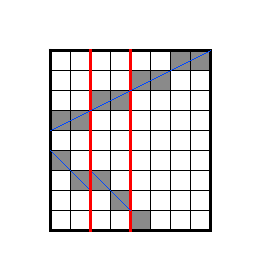
\includegraphics[width=0.4\textwidth]{pattern.png}
  \caption{Диадичные паттерны}
\end{figure}

Например, на рисунке 1, изображены два последовательных рекурсивных разбиения. Рассмотрим второе из них (т.е. то, когда отсекаются два левых столбца). В первой паре столбцов будет найдено два подпаттерна: ПГП с наклоном $t = 0$ и ПГП с наклоном вниз $t = 1$. Во второй паре будет найдено два таких же подпаттерна. Теперь, при объединении этих двух пар столбцов, мы обнаружим две пары подпаттернов, причём верхняя будет иметь сдвиг 1, а нижняя~--- сдвиг 0. При этом, в получившемся изображении ширины 4 будет обнаружено два подпаттерна: ПГП с наклоном вверх $t = 1$ и ПГП с наклоном вниз $t = 3$.

Следует отметить, что потенциальным паттерном считаются только связные последовательности точек, то есть в такой последовательности соседние точки должны иметь общую сторону или угол. При этом, так как ПГП и ПВП рассматриваются по отдельности, такое допущение является валидным, поскольку никакие прямые не будут потеряны.

{\bf Алгоритм быстрого преобразования Хафа}

Перейдем непосредственно к описанию алгоритма БПХ для преимущественно-горизонтальных паттернов с наклоном вверх $(t \in [0, n-1])$. Входом алгоритма является двумерное изображение, а выходом~--- двумерный Хаф-образ, в каждом пикселе которого содержится значение суммы по соответствующему координатам этого пикселя диадическому паттерну.

Входное изображение $I$ рекурсивно разбивается на два равных изображения вертикальной прямой, пока ширина его не будет равна 2. Затем в каждом изображении ширины 2 вычисляются две суммы: левый столбец суммируется с правым поэлементно, после чего правый столбец сдвигается вниз на один пиксель и выполняется второе поэлементное суммирование левого столбца с правым. В результате вычисляются суммы по паттернам длины 2 с наклонами $t = 0$ и $t = 1$. Полученные суммы используются на следующем шаге рекурсии для вычисления сумм по паттернам длины 4 с наклонами $t \in [0; 3]$ в каждой четверке столбцов. Процедура продолжается, пока ширина результирующего изображения не будет составлять $n$.

Оценим вычислительную сложность БПХ. Сумма по всем паттернам длины 2 для пары столбцов требует $2n$ операций, таких пар~--- n/2, для следующего уровня рекурсии требуется $4n$ операций, но четверок на изображении в два раза меньше, чем пар~--- $n/4$, продолжая, получим следующую сумму: \[ 2n \cdot \frac{n}{2} + 4n \cdot \frac{n}{4} + \ldots + n^2, \] а в силу того, что таких слагаемых $\log_2 n$ (по числу уровней рекурсии), окончательно получим оценку сложности $n^2 \log_2 n$. Соответственно, у БПХ для всех типов прямых суммарная сложность будет составлять $4n^2 \log_2 n$.

Таким образом, вычислительная сложность БПХ составляет $O(n^2 \log_2 n)$.

\end{document}
